\documentclass{article}
\usepackage[utf8]{inputenc}
\usepackage{biblatex}
\usepackage{relsize}
\addbibresource{bibliography.bib} %Imports bibliography file
\usepackage{hyperref}
\usepackage{listings}
\usepackage[normalem]{ulem}
\usepackage{float}
\usepackage{graphicx}
\usepackage{svg}
\usepackage{amsmath}
\usepackage{siunitx}
\usepackage{subcaption}
\usepackage{lscape}
\usepackage{booktabs,caption}
\usepackage[flushleft]{threeparttable}

\lstset{
    breaklines=true,
    postbreak=\mbox{\textcolor{red}{$\hookrightarrow$}\space},
    basicstyle=\ttfamily
}

\title{Benchmarking the Tock operating system for embedded platforms \\[0.2em]\smaller{} CSE 221 Project}
\author{Maximilian Apodaca, Grant Jiang, Gabriel Marcano}
\date{\today}

\begin{document}

\maketitle

\section{Introduction}

%Goals of the project
The goal of this project is to measure CPU and memory operations of the Tock operating system \cite{levy17multiprogramming}. The Tock operating system is undergoing a system call interface change, so it would be beneficial to benchmark the original system call interface to form a baseline to compare the new version against. This project provides that baseline, benchmarking CPU and system operations, memory, and inter-process communication facilities on Tock. %https://discord.com/channels/796448392842706954/796448392842706958/801877146548043806

%State the language you used to implement your measurements, and the compiler version and optimization settings you used to compile your code.
Tock is implemented in Rust and supports userspace applications written Rust and C/C++. The benchmarks for this project are written in C. It was considered whether to also implementing the benchmarks in Rust, but this was decided against due to the lack of IPC support from the Rust Tock userspace library.

\subsection{Compilation flags}
The additional flags are used for building the benchmarks on GCC:

\begin{itemize}
    \item \texttt{-O3 -U\_FORTIFY\_SOURCE}
\end{itemize}

By default, the Tock C userspace library, libtock-c, is built using \texttt{-Os}, which tends to prevent inlining in order to save space. For many tests, this lack of inlining added undesired extra overhead, thus the build flags in the libtock-c build system were modified to use \texttt{-O3} instead. One of the computers the team used required the use of the \texttt{-U\_FORTIFY\_SOURCE} flag to build and link with libtock-c, due to that symbol being defined by default on the cross compiler used, which conflicted with other definitions in the userspace library and the newlib (version 4.1.0) standard library the compiler was using. All other flags remained unmodified as declared in the libtock-c build system.

Tock itself was built without modifying any of its default compiler flags. By default, Tock is built in Release mode with debugging symbols. For more information on the build environment and compilers used, refer to section \ref{subsec:versions}.

\subsection{Development}

%If you are measuring in an unusual environment (e.g., virtual machine), discuss the implications of the environment on the measurement task (e.g., additional variance that is difficult for you to control for).
Benchmark application development took place on Linux x86\_64 platforms, leveraging QEMU to simulate the OpenTitan platform, and the final results were acquired by running the benchmarks on an OpenTitan Earl Grey microcontroller instantiation on a Nexys Video Artix-7 FPGA development board \cite{opentitangithub}. Running the tests on the FPGA instead of on QEMU should reduce uncertainty introduced in timing due to QEMU running as a userspace application thus having to share systems resources and time.

Benchmark development was carried out by all team members, and Gabriel Marcano ran the actual experiments on the physical FPGA development board. Table \ref{table:experimenters} lists which benchmarks were done by which team member.

\begin{table}[H]
\centering
    \begin{tabular}{|p{0.30\linewidth}|| p{0.62\linewidth} |}
        \hline
        Maximilian Apodaca & Threading overhead, Task creation timing overhead, Context switch, Kernel memory operations, IPC connection overhead, Size of file cache, File read time\\
        \hline
        Grant Jiang & Loop overhead, RAM access time, IPC round trip time\\
        \hline
        Gabriel Marcano & RAM Bandwidth, Time measurement overhead, Procedure call overhead, System call overhead, IPC peak bandwidth \\
        \hline
    \end{tabular}
\caption{Distribution of benchmarks across team}
\label{table:experimenters}
\end{table}

%Estimate the amount of time you spent on this project.
This project lasted for the duration of the 2020-2021 UCSD Winter quarter (10 weeks). Each team member spent, on average, around 10 hours a week on the project, with longer periods of time near the beginning (to set up the physical hardware) and near the end (to complete the report and tests).

\subsection{Modifications to Tock and user libraries}

Some modifications were necessary for both Tock and user libraries in order to be able to benchmark Tock on the Earl Grey OpenTitan microcontroller. The CPU of the microcontroller does not expose performance counters to userspace, so a new capsule, Perf, was developed to expose two new system calls to get at the lower 32-bits of the cycle counter and instruction count registers. For the purposes of this work, 32-bits of cycle and instruction precision is enough as no timestamp would be more than four billion cycles or instructions apart from another. Also, patches were applied to the Earl Grey platform code in Tock to enable IPC support and to increase the number of memory protection regions Tock is able to manage, which is required for proper IPC usage.

libtock-c, the userspace C library, was modified to add support for the Perf capsule system calls, to facilitate getting the performance data from the kernel. In addition, system call related functions in libtock-c were moved to header files and declared inline in order to allow the compiler, when using optimization level \texttt{-O3}, to inline the system calls and eliminate procedure call overhead.

\section{Machine Description}

\subsection{Hardware}
Table \ref{table:1} summarizes the basic specifications of the OpenTitan Earl Grey microcontroller.

\begin{table}[H]
\centering
    \begin{tabular}{|p{0.36\linewidth}||p{0.55\linewidth}|}
        \hline
        CPU & Ibex RISC-V RV32IMC \\
        \hline
        External Clock & 10 MHz \\
        \hline
        Instruction cache & 4 kiB \\
        \hline
        Data cache & None \\
        \hline
        Pipeline & 3-stage (experimental writeback), variable execution length \\
        \hline
        Branch prediction & None (no penalty for not taken) \\
        \hline
        Memory protection & RISC-V Physical Memory Protection\cite{riscv-priv} \\
        \hline
        Memory regions supported & 16 (1 locked by bootrom) \\
        \hline
        Memory & SRAM, Flash, ROM \\
        \hline
        ROM size & 16 kiB \\
        \hline
        SRAM size & 64 kiB \\
        \hline
        SRAM latency & 1 cycle~\cite{opentitan-latency} \\
        \hline
        Flash size & 512 kiB \\
        \hline
        Interfaces & GPIO, SPI, UART, and JTAG \\
        \hline
        Networking & None \\
        \hline
    \end{tabular}
\caption{OpenTitan Earl Grey Microcontroller specifications}
\label{table:1}
\end{table}

The FPGA bitstream loaded onto the Nexys Video development board implements an OpenTitan Earl Grey microcontroller~\cite{opentitangithub}. The CPU of the microcontroller is an Ibex RISC-V 32-bit CPU (implementing the RISC-V RV32IMC specification), configured to run at 10 MHz, with 4 kiB of instruction cache and no data cache. It has a three stage pipeline consisting of a an Instruction Fetch (IF) stage, followed by an Instruction Decode and Execute (ID/EX) stage (some instructions may spend more than one cycle in the execute stage), and has an experimental writeback stage at the end. As configured for the Earl Grey microcontroller, there is no branch prediction (there is no branch penalty if the branch is not taken). The CPU does not support virtual memory, instead implementing Physical Memory Protection (PMP) per the RISC-V Privileged Specification, version 1.11 \cite{riscv-priv}. The CPU PMP is configured to support up to 16 memory protection regions. There is no floating point unit attached to this CPU.

All of the memory used by the system is kept within the microcontroller; it does not support interfacing with external memory. The microcontroller has 16 kiB of ROM used to store the primary boot loader, 512 kiB of embedded flash (e-flash) to store the actual program data (such as the operating system and application programs and data), and 64 kiB of SRAM as scratch space. SRAM is documented to have a 1 cycle latency to access. The documentation does not state how long it takes to read from ROM or flash ROM, e-flash, and SRAM are mapped to the processors address space and can be accessed directly by the CPU in kernel/machine mode if the PMP is configured to allow access to the right memory regions.

The Earl Grey microcontroller supports GPIO, SPI, UART, and JTAG interfaces to interface with it. Internally, it uses a customized data bus to connect all internal peripherals to the CPU (TLUL bus interconnect). The only peripheral interface used for benchmarking is UART as a way to get program output from the board.

\subsection{Operating system}

The operating system Tock is an "embedded operating system designed for running multiple concurrent, mutually distrustful applications on Cortex-M and RISC-V based embedded platforms"~\cite{tockgithub}. The majority of the operating system is written in Rust, with most parts of the kernel, including all drivers (called capsules), written in safe Rust, and only low level portions hardware specific components written in unsafe Rust and small amounts of assembly language. The kernel uses the Ibex PMP provided by the Earl Grey microcontroller to segregate running userspace applications from each other. Figure~\ref{fig:tock-arch} show the general architecture of Tock.

\begin{figure}[htp]
    \centering
    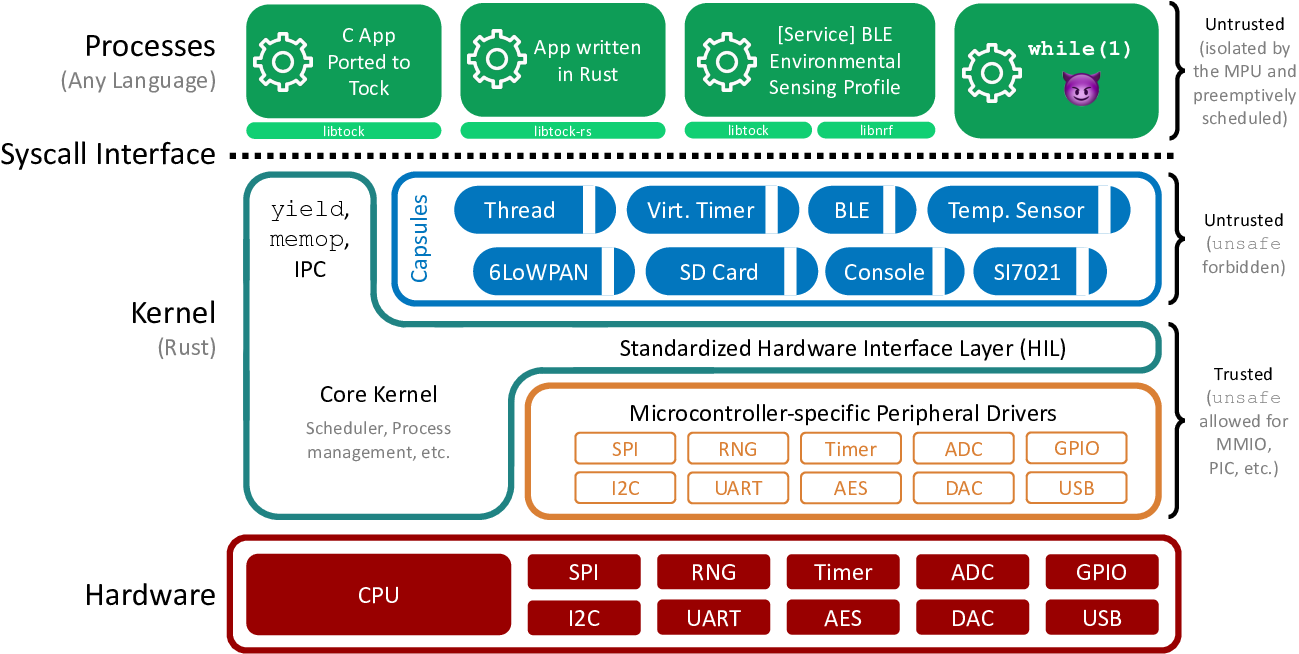
\includegraphics[width=\textwidth]{tock-stack.png}
    \caption{Tock architecture\cite{tockgithub-arch}}
    \label{fig:tock-arch}
\end{figure}

The operating system loads applications from flash on boot, and there is no way currently to load new applications dynamically the initial loading of applications. Applications run preemptively, while kernel level instructions (capsules/drivers and underlying kernel code) execute cooperatively.

\subsection{Versions and builds} \label{subsec:versions}

The Nexys Video FPGA devkit was programmed using the bitstream generated from OpenTitan git commit \texttt{99cb19827} (built using Xilinx Vivado 2020.1), as this is the latest version currently supported by the Tock operating system.

The version of Tock used for benchmarking supports the original, version 1 of the system call interface to the Tock operating system. Specifically, Tock was built using commit \texttt{b2141c0a7} from a fork maintained by the team~\cite{team-tock}. The fork adds IPC support to the Earl Grey board configuration, and adds a performance capsule to allow userspace applications to query the number of retired instruction and the current cycle count.

The compilers and libraries used to build Tock and the benchmarks are shown in table~\ref{table:compilers}. The GCC RISC-V cross-compiler was built using Gentoo Linux's crossdev tool with stack protection disabled (useflag \texttt{-ssp}). Listing \ref{lst:gentoo-riscv} shows the full set of configuration parameters used to build GCC.

\begin{table}[H]
\centering
    \begin{tabular}{|c||c|}
        \hline
        Rust & rustc 1.51.0-nightly (c2de47a9a 2021-01-06) \\
        \hline
        GCC & riscv32-unknown-elf-gcc (Gentoo 10.2.0-r5 p6) 10.2.0 \\
        \hline
        LLVM & LLVM version 11.0.1 \\
        \hline
        libtock-c & 904bef7\cite{team-libtock-c} \\
        \hline
        newlib & 4.1.0 \\
        \hline
    \end{tabular}
\caption{Compilers used for building applications and Tock}
\label{table:compilers}
\end{table}

\begin{lstlisting}[caption={RISC-V RV32 cross-compiler configurations}, label={lst:gentoo-riscv}]
    Using built-in specs.
    COLLECT_GCC=riscv32-unknown-elf-gcc
    COLLECT_LTO_WRAPPER=/usr/libexec/gcc/riscv32-unknown-elf/10.2.0/lto-wrapper
    Target: riscv32-unknown-elf
    Configured with: /tmp/portage/cross-riscv32-unknown-elf/gcc-10.2.0-r5/work/gcc-10.2.0/configure --host=x86_64-pc-linux-gnu --target=riscv32-unknown-elf --build=x86_64-pc-linux-gnu --prefix=/usr --bindir=/usr/x86_64-pc-linux-gnu/riscv32-unknown-elf/gcc-bin/10.2.0 --includedir=/usr/lib/gcc/riscv32-unknown-elf/10.2.0/include --datadir=/usr/share/gcc-data/riscv32-unknown-elf/10.2.0 --mandir=/usr/share/gcc-data/riscv32-unknown-elf/10.2.0/man --infodir=/usr/share/gcc-data/riscv32-unknown-elf/10.2.0/info --with-gxx-include-dir=/usr/lib/gcc/riscv32-unknown-elf/10.2.0/include/g++-v10 --with-python-dir=/share/gcc-data/riscv32-unknown-elf/10.2.0/python --enable-languages=c,c++ --enable-obsolete --enable-secureplt --disable-werror --with-system-zlib --enable-nls --without-included-gettext --enable-checking=release --with-bugurl=https://bugs.gentoo.org/ --with-pkgversion='Gentoo 10.2.0-r5 p6' --disable-esp --enable-libstdcxx-time --with-build-config=bootstrap-lto --enable-poison-system-directories --disable-libstdcxx-time --with-sysroot=/usr/riscv32-unknown-elf --disable-bootstrap --with-newlib --enable-multilib --disable-fixed-point --with-abi=ilp32d --disable-libgomp --disable-libssp --disable-libada --disable-systemtap --disable-vtable-verify --disable-libvtv --without-zstd --enable-lto --without-isl --disable-libsanitizer --disable-default-pie --disable-default-ssp
    Thread model: single
    Supported LTO compression algorithms: zlib
    gcc version 10.2.0 (Gentoo 10.2.0-r5 p6)
\end{lstlisting}

% Measurement overhead: Report the overhead of reading time, and report the overhead of using a loop to measure many iterations of an operation.
\section{Operations and Methodology}

The operations benchmarked for this project are grouped in the following categories:

\begin{itemize}
    \item CPU, scheduling, and OS services
    \item Context switching
    \item Memory access
    \item Inter-process communication
    \item Disk access
\end{itemize}

There is no networking support in the Earl Grey microcontroller.

This section contains the methodologies and results for each of these categories. Benchmarking methods are inspired by the approaches taken by lmbench~\cite{lmbench}.

\subsection{CPU, scheduling, and OS services}

%Measurement overhead: Report the overhead of reading time, and report the overhead of using a loop to measure many iterations of an operation.
\subsubsection{Time measurement overhead} \label{subsubsec:time-measurement}

RISC-V offers performance counters, including a 64-bit cycle counter. The availability of the performance counters from userspace depends on the CPU implementation, and unfortunately the Ibex CPU core used by Earl Grey does not offer access to performance counters from userspace. To work around this limitation, a new module, Perf, was added to Tock to expose a system call to return the lowest 32 bits of the cycle counter. The bottom 32 bits of the cycle counter is sufficient precision to measure all benchmarks in this paper, as no single benchmark sample window is be more than 4 billion cycles (around 429 seconds for the Earl Grey CPU). Listing~\ref{lst:timing_rust} is an example of taking a measurement, in Rust:

%maybe use minted package
\begin{lstlisting}[caption={Timing in Rust},label={lst:timing_rust}]
    let drivers = libtock::retrieve_drivers()?;
    let perf = drivers.perf;
    let timestamp = perf.cycles()?;
    
    // Code to benchmark
    
    let timestamp_end = perf.cycles()?;
    let cycles = timestamp_end - timestamp;
\end{lstlisting}

And listing~\ref{lst:timing_c} is the the same code in C:

\begin{lstlisting}[language=c,caption={Timing in C},label={lst:timing_c}]
    uint32_t timestamp = perf_cycles();
    
    // Code to benchmark
    
    uint32_t timestamp_end = perf_cycles();
    uint32_t cycles = timestamp_end - timestamp;
\end{lstlisting}

Timing measurement overhead sample is acquired by taking two cycle counts in succession. The following C code shows an example:

\begin{lstlisting}[language=c,label={lst:timing_measure},caption={Measuring timing overhead in C}]
    uint32_t timestamp = perf_cycles();
    uint32_t timestamp_end = perf_cycles();
    uint32_t cycles = timestamp_end - timestamp;
\end{lstlisting}

This sample is acquired 1000 times and the results are analyzed to determine the actual overhead. Each sample measures the time it takes for a single Perf system call to complete, and as the Perf capsule system call returns the number of cycles elapsed at the instant the kernel code reaches that particular instruction, the difference in cycles between the first and second cycle counts encompasses the time of the second half of the first system call execution plus the first half of the second system call. Figure \ref{fig:timing} shows a sequence diagram of the process to take a measurement, highlighting the sample window.

\begin{figure}[htbp]
  \centering
  \includesvg[width=0.5\textwidth]{Tock Diagrams - Timing.svg}
  \caption{Timing sequence diagram}
  \label{fig:timing}
\end{figure}

An identical setup is used to collect the number of instructions retired, by replacing \texttt{perf\_cycles()} with \texttt{perf\_instructions\_retired()}. This is used to collect information about how many instructions are executed in a test. Collecting cycle and instruction data is done separately, in order to avoid recording the overhead of one in the other. One caveat of this approach that is not explored in this paper is possible discrepancies between the timing and instruction counts due to kernel preemption taking place in the middle of a sample window.

It is estimated that the timing overhead will be dominated by the system call overhead, as the actual performance majority of the time and cycles spent are in the kernel. Per listing~\ref{lst:tock_perf}, the Perf capsule code in Tock appears well optimized, so the capsule should add extremely little to the system call overhead (a few cycles). It is expected that the number of cycles taken should be around 200 (for around 100 instructions), or 20 microseconds, based on a cursory examination of the RISC-V specific Tock trap and system call code.

\begin{lstlisting}[caption={Tock Perf capsule disassembly}, label={lst:tock_perf}]
    2000288e: addi    a0, zero, 2
    20002890: beq     a1, a0, 18 <2000288e+0x14>
    20002894: addi    a0, zero, 1
    20002896: beq     a1, a0, 18 <2000288e+0x1a>
    2000289a: bnez    a1, 22 <2000288e+0x22>
    2000289c: mv      a0, zero
    2000289e: addi    a1, zero, 1
    200028a0: ret
    200028a2: csrr    a1, minstret
    200028a6: j       6 <2000288e+0x1e>
    200028a8: csrr    a1, mcycle
    200028ac: mv      a0, zero
    200028ae: ret
    200028b0: addi    a0, zero, 11
    200028b2: ret
\end{lstlisting}

For all subsequent tests, timing measurement is done in C using a similar structure as listing~\ref{lst:timing_c}, with the code to be sampled in place of the comment in the listing.

\subsubsection{Loop overhead} \label{subsubsec:loop_overhead}

There are three general loop cases covered by the benchmark, namely:

\begin{itemize}
    \item An empty loop
    \item A loop with a not taken conditional within it
    \item A loop with an alternating conditional within it
\end{itemize}

The goal of the benchmark is to measure the overhead looping introduces and to observe any difference in timing due to differences in branching timing behavior.

Each test scenario involves acquiring 32 samples, with each sample consisting of running a loop 1000 times. The empty loop test consists of an empty for loop, with the only overhead being maintaining a loop counter and branching. The not taken test loop consists of the same overhead as the empty loop plus additional overhead incurred due to an additional branch that should always be not taken. The alternating loop test should be similar to the not taken test loop, except that the internal branch should alternate between taken and not taken for each loop. This is implemented with a ternary operator that tests if the loop counter is odd or even. Special care is taken in the implementation to ensure that the compiler does not optimize out the loops.
%Test 4 has (1 taken, 1 not taken) like test 2 (not taken)

The CPU does not include a branch predictor, but there is a lower performance impact for a branch not taken (at least one less stall cycle), so there is some overhead for every branch taken. It is estimated that the loop overhead on its own (without timing overhead) should be around 4 cycles per loop, or 400 nanoseconds. The second test with the not-taken conditional should add an additional 4 cycles to the loop test overhead for a combined total loop overhead of 8 cycles, or 800 nanoseconds. The third alternating loop test should be similar in structure as the second test, with the added overhead happening due to a cycle stall when branching, so on average this looping should add an additional 2.5 cycles, or 250 nanoseconds, to the overhead, for an overhead of 10.5 cycles per loop, or 1.05 microseconds. All of these estimates are summarized in Table \ref{table:loopestimations}, including the expected measured time for each sample (including timing overhead).

\begin{table}[H]
\centering
    \begin{tabular}{|c||c|c|}
    \hline
    Test        & Overhead per loop (\textmu s) & Estimated sample timing (\textmu s)\\
    \hline
    \hline
    Empty       & 0.400                    & 420\\
    \hline
    Not taken   & 0.800                    & 820\\
    \hline
    Alternating & 1.050                   & 1070\\
    \hline
    \end{tabular}
\caption{Cycle estimations for loops}
\label{table:loopestimations}
\end{table}

%Procedure call overhead: Report as a function of number of integer arguments from 0-7. What is the increment overhead of an argument?
\subsubsection{Procedure call overhead} \label{subsubsec:proc}

The methodology for testing the process call time is to measure the time taken to execute functions with different argument lengths and returns. Specifically, the following set of functions are tested:

\begin{itemize}
    \item An empty procedure with no arguments and no return value
    \item An empty procedure with no arguments and returning a value
    \item An empty procedure with arguments ranging from 1 to 10, returning a value
\end{itemize}

Testing involves measuring the time a single procedure call takes 1000 times, for each kind of procedure being tested. The procedure calls are marked with compiler attributes (specifically \texttt{\_\_attribute\_\_((noinline, optimize(0)))}) to ensure they are not optimized out, so the benchmark actually measures the procedure call cost.

The procedure call overhead should be proportional to the required bookkeeping of registers to save and parameters to pass. Per the RISC-V calling convention~\cite{riscv-calling}, the only registers that must be saved by the callee are registers s0-s11 (the stack pointer is unmodified on a procedure call, and does not need to be saved). Arguments are passed in via the a0-a7 registers for integer values (the Earl Grey CPU core does not support floating point instructions). If there are more than eight arguments, the first eight are passed in via registers, and the remainder are passed in via the stack. Memory latency is supposed to be 1 cycle~\cite{opentitan-latency}, or 100 nanoseconds, thus there should be a small difference between passing arguments via parameters and the stack. Estimates are shown in table~\ref{table:proc}, assuming that a few instructions are required to save and restore instructions. As with all benchmarks, the measured values will also incur timing overhead per sample, which is estimated to be 10 microseconds per sample in section~\ref{subsubsec:time-measurement}.

\begin{table}[H]
\centering
    \begin{tabular}{|c||c|c|}
        \hline
        Test & Overhead (\textmu s) & Total overhead (\textmu s) \\
        \hline
        \hline
        No returns, no parameters & $1$ & $11$ \\
        \hline
        Return, n parameter ($n \leq 8$) & $1.4 + 0.4n$ & $11.4 + 0.4n$ \\
        \hline
        Return, n parameter ($n > 8$) & $4.6 + 0.5(n-8)$ & $14.6 + 0.5(n-8)$ \\
        \hline
    \end{tabular}
\caption{Procedure overhead estimation}
\label{table:proc}
\end{table}

\subsubsection{System call overhead} \label{sec:syscalls}

System calls can be made through libtock-c provided functions, or by manually calling \texttt{ecall} with the right parameters loaded into registers. libtock-c was modified to allow the system call routines to be inlined when compiled with \texttt{-O3}, ensuring that there only overhead being measured is that of the system call itself and not additional overhead introduced by procedure calls.

System call overhead is tested by acquiring 1000 samples, consisting of timestamps before and a system calls to get the current CPU cycle count (with a similar approach for measuring instruction count). The timing overhead is subtracted from the value acquired to get the overhead of a system call. The best system call to use for such a test would be one with minimal overhead, which incidentally would be the same one used for timing as described in section~\ref{subsubsec:time-measurement}.

As the system call being used to benchmark system call overhead is the same as was used for calculating timing overhead, the estimated cycles counts should be the same between this benchmark and the timing overhead test, or roughly, twice the estimated values from section~\ref{subsubsec:time-measurement}, which should be around 40 microseconds or 200 instructions per sample.

\subsubsection{Threading overhead}

Tock does not support multiple threads per process at the present. What the operating system supports in lieu of threads is the ability to subscribe callbacks to be called in the case of events. This takes advantage of Tock's IPC functionality. The profiling of the IPC is discussed in section~\ref{ipc-section}.

\subsubsection{Task creation time}

Tock on the OpenTitan Earl Grey MCU only creates new processes when booting, and there is no way, currently, to create new processes afterwards. Applications are loaded sequentially from flash until all applications are loaded, an invalid application header is found, or the hardware runs out of RAM. After all applications are loaded, the scheduler begins and starts scheduling processes for execution.

\subsubsection{Context switching}

Tock user-level applications are preempted by the kernel scheduler at regular intervals, and scheduled on the Earl Grey platform based on their priority, where the priority is assigned based on load order. Userspace applications can communicate with each other with some IPC facilities provided by the kernel, and thus force a context switch through IPC system calls. As a result the timings for a system call and process switch can be found in section~\ref{sec:syscalls} and section~\ref{ipc-section}.

\subsection{Memory}

The OpenTitan Earl Grey microcontroller has three distinct regions of memory all mapped to the CPU address space: SRAM, flash, and ROM. Only SRAM and flash are accessible from userspace. All tests in this section only benchmark SRAM.

\subsubsection{RAM access time}
% RAM access time: Report latency for individual integer accesses to main memory and the L1 and L2 caches. Present results as a graph with the x-axis as the log of the size of the memory region accessed, and the y-axis as the average latency. Note that the lmbench paper is a good reference for this experiment. In terms of the lmbench paper, measure the "back-to-back-load" latency and report your results in a graph similar to Fig. 1 in the paper. You should not need to use information about the machine or the size of the L1, L2, etc., caches when implementing the experiment; the experiment will reveal these sizes. In your graph, label the places that indicate the different hardware regimes (L1 to L2 transition, etc.).

%[Toshiba94] quotes 110ns as the random read or write cycle time and this time is more representative of the cycle time.
%The ‘‘vacuum’’ means that there is no other activity on the system bus, including no other loads. While this number is frequently used as the memory latency, it is not very useful. It is basically a ‘‘not to exceed’’ number important only for marketing rea- sons.
%When pressed, however, most will admit that cache misses occur in bursts, resulting in perceived latencies of at least the load-in-a-vacuum latency.

%why use and what is backtoback.
%what if it doesn't implement critical word first?
RAM access time is measured by employing the strategy outlined in the lmbench paper for measuring back-to-back-load latency \cite{lmbench}. The lmbench paper measures back-to-back-load ``because it is the only measurement that may be easily measured from software and because we feel that it is what most software developers consider to be memory latency." \cite{lmbench} 

The lmbench paper provides listing~\ref{lst:back-to-back} as an example of how to measure back-to-back-load latency. Specifically, the code causes back-to-back-loads, possibly forcing successive cache misses. Per the paper, some CPUs implement a ``critical word first" optimization where the ``subblock of the cache line that contains the word being loaded is delivered to the processor before the entire cache line has been brought into the cache." \cite{lmbench} If another load is done, with a resulting cache miss, before the previous cache line is completely loaded the cache the CPU must stall the load until that operation completes. The total time between these loads is the back-to-back-load latency. In order to test back-to-back-load latency, then, each access must be approximately the length of the cache line apart.

\begin{lstlisting}[language=c, caption={lmbench back-to-back memory test example}, label={lst:back-to-back}]
    p = head;
    while (p->p_next)
        p = p->p_next;
\end{lstlisting}

%The tests will access memory with 16, 32, and 64 bytes in between.

The specific approach being taken for this benchmark makes no assumption about the cache size of the Earl Grey CPU with the goal to demonstrate that there is, in fact, no data cache. As such, multiple tests are carried out accessing 500 memory locations 16, 32, and 64 bytes apart to show that the behavior does not change regardless of the spacing between data in memory which is expected due to the lack of a data cache.

There is no data cache in the processor so a constant access time should be reported. As there is no data cache, each load and store instruction should complete in a constant number of cycles, ideally 200 nanoseconds per memory access due to 100 nanosecond latency to access memory (one cycle latency)\cite{opentitan-latency}.

%For reference:

% //fill node with junk
% // Goal: each node must be 16/32/64 bytes away from each other, to test for different cache sizes
% // Store cycle count start
% // while looooooooop
% // p->p_next - p > cache line size.
% // Store cycle count end

%Description of back2back benchmark
The benchmark test follows the same design as described by the lmbench which essentially traverses a linked list. For each round of tests, a 500 node linked list is constructed with each node separated from the next by the same number of bytes, or distance. The number of cycles required Then we record the number of cycles it takes to traverse the whole linked list. We estimate accessing each linked list node will take 4 cycles for a total of 2200 cycles including the cycles used for timing or 220 microseconds.


\subsubsection{RAM bandwidth}
% RAM bandwidth: Report bandwidth for both reading and writing. Use loop unrolling to get more accurate results, and keep in mind the effects of cache line prefetching (e.g., see the lmbench paper).
Memory bandwidth is measured in four general approaches, three of which are described by the lmbench paper \cite{lmbench}. The first approach measures copy bandwidth (a combination of read and write bandwidth) by using an existing memory copying routine, in this case \\texttt{memcpy}, to copy buffers from one portion of memory to another. The second approach does a similar test using a simple loop and loads and stores. The third approach measures read bandwidth by reading and summing data in a loop, printing the sum of all values read (to prevent the compiler from optimizing out the memory accesses). The fourth approach measures write bandwidth, by writing a constant value over a large memory buffer with the use of a loop.

Similar to the approach taken in the lmbench paper \cite{lmbench}, all approaches are tested with buffers of different sizes, specifically, all powers of 2 from 32 to 1024, then from 1024 to 16384 in increments of 1024, inclusive. This will help identify any size dependent changes in memory handling, although none are expected. Kernel preemption might be noticeable with larger tests that lake longer to sample.

Per the OpenTitan SRAM documentation, SRAM access has a latency of once cycle\cite{opentitan-latency}, so assuming SRAM reads and writes take two cycle per word access total, optimally, both read and write bandwidths should be close to 20 MB/s or 19.1 MiB/s, as the CPU clock is 10MHz. Estimating overhead is difficult, since SRAM access latency is lower than all sources of overhead. Looking at the generated assembly of the tests indicates that at least some of the measurements are unrolled completely, in which case the only source of overhead would be timing related, which is estimated to be 20 \textmu s. For all other tests involving loops, the overhead is estimated to be 20 \textmu s plus the loop overhead estimation of 0.4 \textmu s times the number of times the loop executes.

%Realistically, overhead from using the CPU to copy memory, in the form of looping, is going to reduce bandwidth appreciably. Using the estimates from section \ref{subsubsec:loop_overhead} of 0.4 \textmu s per loop iteration, and estimating 0.2 \textmu s per word access on average, it should take 2457.6 \textmu s to copy 16 KiB, which translates to a bandwidth of 6.67 MB/s.

\subsubsection{Kernel memory operations}
% Page fault service time: Report the time for faulting an entire page from disk (mmap is one useful mechanism). Dividing by the size of a page, how does it compare to the latency of accessing a byte from main memory? 
The Tock operating system does not support virtual memory and thus has no concept of page faults \footnote{There is a pending pull request with similar functionality at \url{https://github.com/tock/tock/pull/2424}}. However, it does support some memory-related system calls. The brk and sbrk memop system calls alter the memory layout, specifically the application boundary, of the current application. Benchmarking brk and sbrk should yield timing about adjustments to memory protection regions.

Testing involves sampling 1000 times, where each sample makes a \texttt{setbrk} system call to increase the memory break point by 8 bytes every sample.

It is estimated that each system call for brk and sbrk will take roughly double the amount of time to get the timer count (\ref{subsubsec:time-measurement}), due to the overhead in updating kernel internal structures and the memory protection unit registers. This translates to 40 microseconds per \texttt{setbrk} system call, or 60 microseconds with timing overhead included per sample.

\subsection{Inter-process communication (IPC)} \label{ipc-section}

While Tock does support UDP on IPv6, the Earl Grey microcontroller has no networking hardware. In lieu of testing network round trip time, peak bandwidth, and connection overhead, similar tests were implemented over IPC.

The IPC implementation in Tock is based on a client server abstraction. A server can register itself as a service that clients can look up, and both client and server can register callbacks with the IPC driver to be called when notified by the other. In addition, each process can optionally allocate a shared memory buffer which is passed to the callback belonging to the other application.
% A server process can register a callback with the kernel. This callback is invoked when a client process notifies the server. This is most analogous to a multi-threading environment since we have an effective mechanism to synchronize multiple programs. In addition, client processes have the option to allocate a shared memory buffer which is passed to the server. This allows for shared memory multi-threading.

The methodology to measure the IPC overhead involves taking the time it takes to signal a process from another. This is done by creating a loop where the client notifies the server, and then the server notifies the client again. The server writes the current timestamp to a shared buffer owned by the client and notifies the client. The client then subtracts the current timestamp from the timestamp written into the shared buffer. This measures the time it takes to switch a single context from the server to the client.

The measurements are repeated in four different cases. The first is a client notifying the server to analyze how long it takes to switch from client execution to server execution. The next is a server switching to the client to measure the time it takes to switch from the server execution to the client execution. The third is measuring the round trip time which should be the sum of both of the uni-directional switches. Finally, the overhead of establishing a connection is measured by having the client find (and fail to find) an IPC service.

During most of the testing a shared buffer is allocated on the client side. This results in one extra entry in the memory protection unit for the server. As a result it is expected that switching to the server will take slightly longer than switching to the client. Overall, it is estimated that an IPC invocation will take 20 times as long as a system call, or 800 microseconds. This approximately due to the of the length of code observed in the Tock kernel to handle these tasks.

The round trip time is the amount of time between the client sending and receiving a reply from a server. After a ping is received, the time elapsed is recorded, and then the next ping gets sent. The estimated round trip time is 1.6 milliseconds, or twice the estimate for a one way communication.

The connection overhead is the overhead required by applications to find an existing IPC service running under Tock. The server application registers itself with Tock as an IPC server, and the client application does a IPC service lookup. The benchmark measures the amount of cycles required to find the server, and the amount of time required to fail to find a server (by using a bad service name).

It is estimated that the connection overhead should be equal to that of a system call plus the cycles required to update kernel structures to establish a client with the server, which should be in the order of another system call. As such, it should take around 400 cycles or 40 microseconds to find an establish a connection with an IPC service.

\begin{figure}[htbp]
  \centering
  \includesvg[width=0.8\textwidth]{IPC-Communication-Flowchart.svg}
  \caption{The IPC flow employed for the IPC tests.}
\end{figure}

% We don't have a network connection. This might be a good time to profile the inter process communication framework instead. Here we can measure the time it takes to "transmit" and "receive" data from another process.

% \^This is a lie

\subsubsection{Peak bandwidth}

The testing methodology involves the client application setting up a 10 kiB buffer, recording an initial timestamp, and then sharing the buffer with the server and sending a notification to the server to wake it up. The server then wakes up, and reads the 10 kiB buffer, and records a timestamp once it is finished. It then sends another notification to the client along with its timestamp, so the client can compute the number of cycles elapsed. Figure~\ref{fig:ipc_bandwith} shows a graphical representation of the test.

\begin{figure}[htbp]
  \centering
  \includesvg[width=0.8\textwidth]{IPC Bandwidth.svg}
  \caption{Sequence diagram of client server operations for IPC bandwidth test}
  \label{fig:ipc_bandwith}
\end{figure}

It is estimated that each sample will take 1.884 ms, which consists of the timing overhead, one system call, one context switch, and coping 10 kiB of memory. The without the timing overhead, if everything else is considered part of the bandwidth computation, should take 1.864 ms, which translates to about 5.5 MB/s or 5.2 MiB/s for bandwidth.

\subsection{File system}

Tock does not provide any native filesystem support, but it does provide applications access to raw flash memory, where program code resides. Each application is able to read (but not modify) its own program flash memory. However, due to a bug in the flash controller in the Earl Grey processor applications are unable to write to flash.\footnote{Interrupts do not appear to update status bits: https://github.com/lowRISC/opentitan/issues/4730}

\subsubsection{Size of file cache}
% Size of file cache: Note that the file cache size is determined by the OS and will be sensitive to other load on the machine; for an application accessing lots of file system data, an OS will use a notable fraction of main memory (GBs) for the file system cache. Report results as a graph whose x-axis is the size of the file being accessed and the y-axis is the average read I/O time. Do not use a system call or utility program to determine this metric except to sanity check.
Tock does not have a file system and therefore does not have a file cache. However the CPU core does have an instruction cache. Since instructions are fetched directly from flash the effective file cache can be profiled by examining the instruction cache performance.

To measure the size of the instruction cache a loop is created with a variable number of NOPs. By adjusting the number of NOPs generated the time it takes to complete a loop is affected. If the time it takes to load each NOP is the same then the time for a loop iteration will increase linearly. However, there should be a change in performance when the instruction cache is saturated, leading to an increase in the time per instruction, thus yielding a different slope for the time increase data. Figure~\ref{nop-diagram} illustrates the placement of the NOPs and program flow.

\begin{figure}[htbp]
  \centering
  \includesvg[width=0.5\textwidth]{Tock Diagrams - Nop diagram.svg}
  \caption{The layout of the test function in memory with two different NOP chain lengths.} \label{nop-diagram}
\end{figure}

Based on reading the parameters used to build the Earl Grey bitstream by the OpenTitan project, the instruction cache is 4 kiB in size. This means that after 2048 NOPs (as each NOP is a two byte instruction) in the loop there should be a change in the time per NOP in each iteration. The slope of the measurements should be one cycle per instruction until the 2048th NOP is reached, at which point we expect every 64 NOPs to evict an existing 64 NOPs. The expected slope would be around two cycles 200 nanoseconds per instruction.

\subsubsection{File read time}
% File read time: Report for both sequential and random access as a function of file size. Discuss the sense in which your "sequential" access might not be sequential. Ensure that you are not measuring cached data (e.g., use the raw device interface which bypasses the file system (see "man lsblk" if you are using Linux). Report as a graph with a log/log plot with the x-axis the size of the file and y-axis the average per-block time.
% The instruction cache could affect this as flash bandwidth is shared. It would be interesting to measure the read time. We can do this and it should give clean results. We don't have to worry about any caches as our program reads directly from the device.
Since Tock does not support a filesystem, but it does expose the memory mapped flash regions of each application to the application as read-only memory. As an alternate test, the flash read bandwidth should provide a proxy of low-level filesystem performance, were once implemented for Tock. A simple loop that reads a continuous region from flash as well as a loop that does random four byte accesses are used to measure flash read performance. The expected throughput for flash operations is the same 20 MiB/s as for SRAM operations as they supposedly share the same SRAM backing in the FPGA. There should also be a 25\% overhead for doing the sparse access due to the increased amount of computation per access. It is not possible to test file write as memory mapped regions of flash are mapped read only to userspace applications.

\subsubsection{Remote file read time}
% Remote file read time: Repeat the previous experiment for a remote file system. What is the "network penalty" of accessing files over the network? You can either configure your second machine to provide remote file access, or you can perform the experiment on a department machine (e.g., APE lab). On these machines your home directory is mounted over NFS, so accessing a file under your home directory will be a remote file access (although, again, keep in mind file caching effects).
This test is not done as there is no networking support.

% Contention: Report the average time to read one file system block of data as a function of the number of processes simultaneously performing the same operation on different files on the same disk (and not in the file buffer cache).
\subsubsection{Contention}
% We can do this for userspace applications however capsules use a cooperative multiprocessing environment and might give interesting results. We would expect throughput to be slightly less than 1/N * memory bandwidth for each process. 
This test is not done as there is no filesystem to content over.

\section{Measurements and discussion}

All the tests were implemented in C using libtock-c. Each test consisted of many samples which were then averaged together to produce results.

One of the most striking features of all of the results is that the timing was extremely deterministic. This was expected to some extent, as the Earl Grey microcontroller does not perform speculative execution and only offers a single execution pipeline, but not to the extent manifested. For all tests performed, the difference between samples was zero, meaning the standard deviation of each individual test was zero. It is hypothesized that using \texttt{printf} right after each sample window, which invokes a \texttt{yield} system call returning control to the kernel for some time, could reset the timeslice allocated for the application, so every sample loop, so long as it's short enough, is able to run uninterrupted.

It was more difficult than expected to interpret measurements due to the Earl Grey microcontroller's CPU implementation enabling a highly experimental feature adding a third pipeline stage for writeback. The documentation for the Ibex CPU core states that all performance descriptions in the documentation are relevant only for a two stage instantiation and that performance will be different with all three stages enabled\cite{ibex-pipeline}.

\subsection{CPU, scheduling, and OS Services}

\subsubsection{Time measurement overhead} \label{subsubsec:time_measurement_overhead_meas}

Table~\ref{table:time_measurement} shows the summary of the time measurement overhead.

\begin{table}[H]
\centering
    \begin{tabular}{|c||c|c|}
        \hline
        & Time (\textmu s) & Instructions \\
        \hline
        \hline
        Estimated & 20 & 100\\
        \hline
        Actual & 226.8 & 844\\
        \hline
    \end{tabular}
\caption{Time measurement overhead}
\label{table:time_measurement}
\end{table}

Timing overhead is measured to be 226.8 microseconds, or 844 instructions. This is significantly higher than the 20 microseconds that was estimated by an order of magnitude. As Listing \ref{lst:tock_perf} shows, the actual capsule driver implementation in Tock itself reduces to a fast dispatch and a single instruction for reading from the counter. This implies that something else in the kernel is taking a much larger number of instructions than expected before finally invoking the Perf capsule routines. The original estimate was based on a cursory overview of the Tock trap handler and context switching code for the RISC-V architecture, which have roughly 100 assembly instructions combined.  This overhead should be equal to the one calculated in the system call overhead section, in section \ref{subsubsec:system_call_overhead}.

Listing \ref{timing_dis} shows the relevant instructions used from userspace to set up the timing system call and to call it once again, which consists of the actual test. Before this code listing the program sets up the s2 register with the Perf capsule driver number to pass to the system call (0x00090004). Of note, the critical test portion is the section between and including the two \texttt{ecall} instructions, showing that GCC was able to inline the system calls adequately. This means all of the overhead measured is taking place inside the kernel.

\begin{lstlisting}[caption={Timing overhead benchmark disassembly}, label={timing_dis}]
    20030148:       mv      a1,s2
    2003014a:       li      a2,1
    2003014c:       li      a3,0
    2003014e:       li      a4,0
    20030150:       li      a0,2
    20030152:       ecall
    20030156:       mv      a5,a0
    20030158:       li      a0,2
    2003015a:       ecall
    2003015e:       mv      a1,s0
    20030160:       sub     a2,a0,a5
    20030164:       addi    s0,s0,1
    20030166:       addi    a0,s1,184 # 2003a0b8
    2003016a:       auipc   ra,0x7
    2003016e:       jalr    42(ra) # 20037194 <printf>
    20030172:       bne     s0,s3,20030148
\end{lstlisting}

\subsubsection{Loop overhead} \label{subsubsec:loop_overhead_meas}

Table~\ref{table:loop-overhead} details the benchmark results for timing loops with different branches. The estimates of the amount of time taken for each of the loop tests are quite off compared to the actual timings, possibly due to the uncertainty in CPU timing due to the experimental CPU pipeline stage effects. Specifically, the difference in the estimates and the actual measured values is likely due to not understanding the specific delays for loads and stores and for branch taken, even though the documentation suggests SRAM has a latency of one cycle.

\begin{table}[htp]
\centering
\begin{tabular}{|c||c|c|c|}
 \hline
 Loop Type & Raw time & Estimated overall & Loop portion \\
 \hline\hline
 Empty Loop & 0.7271ms & 0.42ms & 0.5003ms\\
 \hline
 Always not taken & 1.1269ms & 0.82ms  & 0.9001ms\\
 \hline
 Alternating Loop & 2.2257ms & 1.07ms  & 1.9989ms\\
 \hline
\end{tabular}
\caption{Time of each loop test (1000 loops)}
\label{table:loop-overhead}
\end{table}
%1ms = 10,000cycles; sram latency is 1clock cycle

%Does it just do nothing for adds?

%Documentation: https://ibex-core.readthedocs.io/en/latest/03_reference/pipeline_details.html?highlight=pipeline

The documentation states that integer instructions do not stall and that the branch taken will stall by at least once cycle, subject to memory latency for fetching the new instruction. Looking at the generated assembly, for the second and third test there are extra instructions emitted to set up the inner branches that the estimates did not take into account.

%It seems odd that empty and always not taken are so similar yet the alternating loop is so much larger (11557 cycles. geez lol)
%empty4=5000, nottaken8=9000, alternating10.5=19,989

%empty4:         addi(1), bne taken(4), total 5
The for loop in the empty loop test is compiled to an add immediate and a branch taken. Together these take at least 2 non stalling cycles. The empty loop test reports 0.5003ms which indicates each loop iteration takes approximately 5 cycles or 500 nanoseconds. It is hypothesized that the extra three cycles are due to branch stalling in the pipeline.

%Doesn't stalling once mean only 1 cycle is wasted (on a branch taken) so it probably should be stall 3 cycles?
%     1   2   3   ... 4   5   6   7
% add IF  EX  WB
% bne     IF  EX  ... WB
% ...         IF
% add             ... IF

%always not9:    lw(3), addi(1), bnez not taken(1), bnez taken(4)
The assembly of the for loop for the always not taken test consists of a load word, add immediate, branch not taken, and a branch taken. The always not taken test reports 9001 microseconds which indicates each loop iteration takes approximately 9 cycles to complete, or 900 nanoseconds. Each loop consists of 4 instructions with the branch taken stalling for three cycles. This hints the load stalled for two cycles, in accordance with findings from section~\ref{subsubsec:ram_acces_time}.

%alternate :    loop1: andi1, bnez taken4,     lw3, addi1, addi1, sw3, bne taken4
%               loop2: andi1, bnez not taken1, lw3, addi1, addi1, sw3, bne taken
%combined:
% andi1, lw3, addi1, addi1, sw3, taken4
%     + nottaken3/taken4
%I get 13/14 cycles/loop. Missing 5/6 cycles/loop
The alternating loop test alternates based on parity of the loop counter which increments by 1. The test reports it used 19989 cycles or approximately 19 cycles per loop. Unfortunately, it was not possible to correlate each estimated instruction with the cycles per loop. For each loop iteration, regardless of the loop counter's parity, the loop consists of an and immediate, a load word, 2 add immediates, a store word, and a branch taken. This accounts for 13 cycles, 7 of which are stalls. When the loop counter is even, there is an additional branch taken taking 4 cycles. When the loop counter is odd, there is an additional branch not taken taking 1 cycle. This accounts for an average of 15.5 cycles per loop iteration. This leaves 3.5 cycles per loop iteration unaccounted for. It is possible that the load and store word instructions stall for more time, or there are other pipeline effects caused by the experimental writeback stage being enabled.

%diff b/w alwaysnot and alternate: to account for about 11000 cycles
%andi, addi, sw, bnez taken. Always not has a b not taken
%andi, addi, sw, 
%and/add take 2 cycles, sw takes 3, 

\subsubsection{Procedure call overhead}

Figure \ref{fig:proc} shows the procedure call measurements as a function of how many arguments and returns are handled, and figure \ref{fig:proc_est} shows the estimated values, for comparison. Note the scale of the y axis is not the same for both graphs. To clarify the values in the x axis, they represent the different tests as explained in section~\ref{subsubsec:proc}, beginning with an empty procedure, then a procedure with no arguments but now returning a value, and then procedures with the given number of arguments.

\begin{figure}[hp]
    \centering
    \begin{subfigure}[b]{1\textwidth}
        \centering
        \includesvg[width=.9\textwidth]{Procedure_call_benchmark_cycles_estimated.svg}
        \caption{Estimates, including overhead}
        \label{fig:proc_est}
    \end{subfigure}
    \begin{subfigure}[b]{1\textwidth}
        \centering
        \includesvg[width=.9\textwidth]{Procedure_call_benchmark_cycles.svg}
        \caption{Measurements, with overhead}
        \label{fig:proc}
    \end{subfigure}
    \caption{Procedure call measurements and estimates}
\end{figure}

The estimated values were offset mostly due to the timing overhead estimation being incorrect (see section~\ref{subsubsec:time_measurement_overhead_meas}). A linear regression on the data used to generate both figures revealed the slope of figure~\ref{fig:proc} to be 0.375 \textmu s, and of figure~\ref{fig:proc_est} to be 0.411 \textmu s, which translates to a difference of less than a cycle per additional parameter between the estimates and the measured values.

Of note, it is not clear why there is a drop in time between the plain or void function test and the return function test, as the only difference is that the latter is actually returning a value and the former is not. In fact, looking at the instruction counts in figure~\ref{fig:proc_inst}, the return function test does execute more instructions. Other than this anomaly, the rest of the graph is more or less as expected. Due to low SRAM latency, there is not a drastic in performance between the 8 parameter and 9 parameter test. In fact the change appears to be in the opposite direction as expected, although slight, showing a smaller increase in time for adding the 9th parameter. Looking at the assembly code generated, that might be simply because the test function does not have to restore any registers related to the 9th and beyond, thus no overhead is generated on a return for those extra arguments, just on procedure call to pass the parameters.

\begin{figure}[htp]
    \centering
        \includesvg[width=.9\textwidth]{Procedure_call_benchmark_instructions.svg}
        \caption{Procedure call measurements, instruction count}
        \label{fig:proc_inst}
\end{figure}

\subsubsection{System call overhead} \label{subsubsec:system_call_overhead}

%  In the table report the base hardware performance (when applicable), your estimate of software overhead, your prediction of operation time, and your measured operation time. For units, use wall-clock time (e.g., microseconds) instead of cycles.

The actual operation values were computed by subtracting the time measurement overhead, shown in table \ref{table:time_measurement} from the measured results. These computed results are shown at the end of table \ref{table:system_call_overhead}.

\begin{table}[htp]
\centering
    \begin{tabular}{|c||c|c|}
        \hline
        Measurement type & Time (\textmu s) & Instructions\\
        \hline
        \hline
        Estimated overhead & 20 & 100 \\
        \hline
        Estimated operation & 20 & 100 \\
        \hline
        Measured & 453.5 & 1690 \\
        \hline
    \end{tabular}
\caption{System call overhead}
\label{table:system_call_overhead}
\end{table}

The estimates are as inaccurate as they were for section \ref{subsubsec:time_measurement_overhead_meas} and for the same reasons, as the test is using the same system call for the code being tested as is used for timing purposes. The estimate predicted that the overhead and the operation should both be the same amount of time, and that does show in the actual data collected, noting that the measured data is almost exactly double the measured time for the time measurement overhead in section \ref{subsubsec:time_measurement_overhead_meas}.

\subsection {Memory}

\subsubsection{RAM access time} \label{subsubsec:ram_acces_time}

%latency is 1 cycle for SRAM per https://docs.opentitan.org/hw/ip/sram\_ctrl/doc/

%estimated accessing each linked list node will take 4 cycles for a total of 2200 cycles including the cycles used for timing or 220 microseconds. Actual is 6271 cycles

The measurements taken for the RAM access time test are all 627.1 \textmu s exactly, regardless of the back-to-back distance employed. Without the overhead of recording the cycle counts and 500 loops, the actual memory accesses should take somewhere around 150.3 \textmu s for 500 accesses, indicating a single load word instruction is around 300 ns or 3 cycles, implying a latency of two cycles instead of the one cycle latency predicted and expected per the platform documentation.

The back-to-back latency test would have reported a difference in across some of the tests if a small data cache were in use, thus the lack of variability across different distances tested indicates that there is not a data cache employed, consistent with known hardware specifications.


%just lw and b taken instructions per node traversal. Unless lw also stalls for 3 cycles, it doesn't add up.

\subsubsection{RAM bandwidth}

Figure~\ref{fig:bandwidth_time} shows the time required to complete each test with different size buffers, along with the estimated time for the ideal case. Figure~\ref{fig:bandwidth_instr} shows the number of instructions required to complete each test with different size buffers.

\begin{figure}[hp]
    \centering
    \begin{subfigure}[b]{1\textwidth}
        \centering
        \includesvg[width=.9\textwidth]{bandwidth_benchmark_cycles.svg}
        \caption{Timing measurements}
        \label{fig:bandwidth_time}
    \end{subfigure}
    \begin{subfigure}[b]{1\textwidth}
        \centering
        \includesvg[width=.9\textwidth]{bandwidth_benchmark_instructions.svg}
        \caption{Instructions measurements}
        \label{fig:bandwidth_instr}
    \end{subfigure}
    \caption{RAM bandwidth measurements and estimates}
\end{figure}

Memory bandwidth was difficult to compute from the measured data, as memory overhead is significantly lower than timing overhead and close to the same as looping overhead. As a result, overhead comprises a non-negligible amount of the measurements. Figure~\ref{fig:bandwidth_time} shows that all measured tests were appreciably slower than the ideal estimate, by comparing the rate of increase in time as the buffer size increased. The effect of the overhead can be seen in figure~\ref{fig:bandwidth_instr}, where there is a clear correlation between the faster tests in figure~\ref{fig:bandwidth_instr} requiring a lower number of instructions.

One observation from looking at both figures is that while the instructions required as a function of buffer size appear extremely linear, the times reflected in figure~\ref{fig:bandwidth_time} for some tests show some noise or jitter. It is speculated that for the larger buffer sizes each test takes long enough to be occasionally preempted by the operating system kernel, leading to increases in time. It is strange that the spikes did not manifest themselves as noise in the actual data collection, but only when looking at tests of different sizes. This quirk is possibly due to how deterministic the timing of the test environment is due to the test being the only application executing on the operating system, and that there  are not many interrupts firing in the background, other than the timer interrupt which should be consistent, if not deterministic.

In lieu of trying to extract a bandwidth measurement from the figures, a study of the the generated assembly for some of the tests discovered that GCC successfully inlined some of the memcpy and manual memory copy loops, and that generally it had more success inlining memcpy than the manual memory copy approach. Moreover, GCC was able to also eliminate all looping for small copy amounts. An upper bound for the memory bandwith was computed using the average of the data from this optimized GCC memcpy, where it copied 32 bytes of data without looping. Table \ref{table:ram_bandwidth_memcpy} shows the estimates and the measured time of the memcpy test. Assuming timing overhead is consistent and the same as in section \ref{subsubsec:time_measurement_overhead_meas}, the actual time to copy 32 bytes (read 32 bytes and write 32 bytes) was 4.4 \textmu s, which translates to a bandwidth of 14.5 MB/s or 13.9 MiB/s.

GCC supports pragmas to instruct it to unroll loops explicitly, but it did not seem possible to force GCC to unroll the loops father than some set constant. It is hypothesised that this limit might be related to the immediate offset range in the lw and sw operations, but this was not verified.

\begin{table}[H]
\centering
    \begin{tabular}{|c||c|c|}
        \hline
        Measurement type & Time (\textmu s) & Instructions\\
        \hline
        \hline
        Estimated overhead & 20 & 100 \\
        \hline
        Estimated operation & 12.8 & 16 \\
        \hline
        Measured & 231.2 & 860 \\
        \hline
    \end{tabular}
\caption{System call overhead}
\label{table:ram_bandwidth_memcpy}
\end{table}

The findings from this test go slightly counter to the observations from section~\ref{subsubsec:ram_acces_time}, where if SRAM latency is two cycles instead of one, the theoretical maximum bandwidth should be capped at 13.3 MB/s or 12.7 MiB/s. It is not clear what could be causing this discrepancy and memory benchmarks should definitely be re-visited in the future to help identify the actual hardware performance, as the documentation is incomplete in the presence of the experimental writeback pipeline stage.

\subsubsection{Memory Protection Update}

The set break system call was used to measure the time a memory protection update takes. This system call allows the program to set the program break, which forces an update of the memory protection regions and therefore allows us to measure the overhead of updating the MPU regions. The predicted a 0.45 milliseconds overhead per call to break was different than the measured amount 0.65 milliseconds. This is reasonably close to the correct value especially since if the actual measurement overhead is subtracted from the actual measurement overhead the result is 0.42 microseconds, which is much closer to the estimated value. If the system call overhead is subtracted from this processed value, the result is 197.4 microseconds to update the MPU regions. It is of note that a quick review of the Tock code to update memory regions appears to indicate a complexity of $O(n)$ per update, where n is the number of regions. This test only operates with $n = 2$. Table~\ref{table:mem-overhead} shows the measured and estimated times in addition to the measured time minus our measurement overhead.

\begin{table}[h!]
\centering
\begin{tabular}{|c||c|} 
 \hline
 Timing type & Time (ms) \\
 \hline
 \hline
 Estimated & 0.4536\\
 \hline
 Processed & 0.4242\\ 
 \hline
 Measured & 0.6510\\
 \hline
\end{tabular}
\caption{Time taken by memory system call.}
\label{table:mem-overhead}
\end{table}

\subsection{Inter-process communication}

\begin{table}[h!]
\centering
\begin{tabular}{|c||c|c|c|} 
 \hline
 Direction & Raw Time & Processed Time & Estimated Time \\ [0.5ex] 
 \hline\hline
 Client to Server & 2.1600 \si{\milli\second} & 1.9332 \si{\milli\second} & 5 \si{\milli\second} \\ 
 \hline
 Server to Client & 2.6595 \si{\milli\second} & 2.4327 \si{\milli\second} & 4.5 \si{\milli\second} \\
 \hline
 Round Trip & 4.6883 \si{\milli\second} & 4.4615 \si{\milli\second} & 9.5 \si{\milli\second} \\
 \hline
 Connection overhead (success) & 0.6823 \si{\milli\second} & 0.4555 \si{\milli\second} & 0.0400 \si{\milli\second} \\
 \hline
 Connection overhead (failure) & 0.6530 \si{\milli\second} & 0.4262 \si{\milli\second} & 0.0400 \si{\milli\second} \\[1ex] 
 \hline
\end{tabular}
\caption{IPC Communication overhead}
\label{table:ipc-overhead}
\end{table}

The IPC communication delay was measured to be on average 2.18 \si{\milli\second}. This differs from our expected 4.75 \si{\milli\second} estimate by over 2.2x. The most likely cause for the discrepancy is poor estimation of the amount of instructions needed to execute. However, another reasonable assumption is that the MPU context switch is faster than expected.

We predicted the client to server communication would take longer as an extra region has to be mapped into the server's address space before the server can execute. However the client to server context switch took less time than the server to client switch. This might be due to the way Tock prioritizes processes. The server is loaded first which might give it priority over the client. This means that when the client contacts the server, the server runs immediately. But when the server contacts the client, control is transferred back to the server, and only after the server yields does the client run.

The round trip time should be a sum of the client to server and server to client times. However the sum gives 4.3659 \si{\milli\second} which is 95.6 \si{\micro\second} short. This is at most 956 instructions\cite{ibex-pipeline} and represents less than a system call as shown in table~\ref{table:time_measurement}. As a result we believe the discrepancy is due to some extra checks the scheduler does to determine what process to schedule.

\subsubsection{Peak Bandwidth}

Table~\ref{table:ipc_bandwidth_meas} shows the results from measuring IPC bandwidth. Of note, this is the only test where the first data sample differed from all others. This makes sense as the buffer sharing is set up only at the beginning, and due to optimizations deep in the Tock kernel if a requested section is already in place no further work needs to be done to share a buffer.

\begin{table}[H]
\centering
    \begin{tabular}{|c||c|c|}
        \hline
        Measurement type & Time (\textmu s)\\
        \hline
        \hline
        Estimated overhead & 20\\
        \hline
        Estimated operation & 1864\\
        \hline
        Measured (first) & 4060.0\\
        \hline
        Measured (steady)& 3960.8\\
        \hline
    \end{tabular}
\caption{IPC bandwidth test timing}
\label{table:ipc_bandwidth_meas}
\end{table}

If overhead is just the timing measurement, using data from section~\ref{subsubsec:time_measurement_overhead_meas} the actual operation should have taken 3833.2 microseconds for the first sample and 3734.0 microseconds for all others. Both of these are double the estimated operations. The previous IPC results for a one way trip from the client to server takes around 2.1 milliseconds, leaving around 1.6 milliseconds to copy the data on the server side which is likely more than enough to copy 10 kiB of data, even including looping overhead. It appears IPC mechanisms take significantly more than just a context switch. Using the second case as the best case for bandwidth, and after substracting the actual measurement overhead from the measured test, the bandwidth is 2.7 MB/s or 2.6 MiB/s, which is about half of the estimated bandwidth.

\subsection{Filesystem}
\subsubsection{Flash Access}

\begin{table}[h!]
\centering
\begin{tabular}{|c||c|c|c|} 
 \hline
 Type & Throughput & Estimate & Overhead \\ [0.5ex]
 \hline\hline
 Sequential & 1.968 MiB/s & 20 MiB/s & 0.125 instr/load \\
 \hline
 Sporadic & 1.396 MiB/s & 15 MiB/s & 8 instr/load \\ [1ex] 
 \hline
\end{tabular}
\caption{Flash bandwidth and loop overhead}
\label{table:flash-bandwidth}
\end{table}

Flash bandwidth was measured as an analog to reading a file from a filesystem. It was expected that the performance would be similarly to SRAM access since it was expected that the FPGA implementation might not be using real flash memory as it is lost on power loss. However, there was a much lower performance measured, possibly due to a difference in micro-architecture for handling flash and memory accesses.

\begin{lstlisting}[caption={Sequential flash copy disassembly}, label={seq_flash}]
    20030198:	4398              lw	a4,0(a5)
    2003019a:	43d8              lw	a4,4(a5)
    2003019c:	4798              lw	a4,8(a5)
    2003019e:	47d8              lw	a4,12(a5)
    200301a0:	4b98              lw	a4,16(a5)
    200301a2:	4bd8              lw	a4,20(a5)
    200301a4:	4f98              lw	a4,24(a5)
    200301a6:	4fd8              lw	a4,28(a5)
    200301a8:	5398              lw	a4,32(a5)
    200301aa:	53d8              lw	a4,36(a5)
    200301ac:	5798              lw	a4,40(a5)
    200301ae:	57d8              lw	a4,44(a5)
    200301b0:	5b98              lw	a4,48(a5)
    200301b2:	5bd8              lw	a4,52(a5)
    200301b4:	5f98              lw	a4,56(a5)
    200301b6:	04078793          addi	a5,a5,64
    200301ba:	ffc7a703          lw	a4,-4(a5)
    200301be:	fd479de3          bne	a5,s4,20030198
\end{lstlisting}

A sequential read test was done by unrolling a loop reading 16 values from flash at a time. This unrolled loop was measured by acquiring the number of cycles before and after the loop. The code listing~\ref{seq_flash} shows the assembly generated by the loop. This shows that there are 2 instructions overhead for every sixteen loads. It was expected that this value to not greatly affect the bandwidth and therefore do not report corrected values.

\begin{lstlisting}[caption={Sporadic flash copy disassembly}, label={spo_flash}]
2003026c:	054cec63          bltu	s9,s4,200302c4 
...
200302c4:	000ca783          lw	a5,0(s9)
200302c8:	0405              addi	s0,s0,1
200302ca:	9d3e              add	s10,s10,a5
200302cc:	07f7f793          andi	a5,a5,127
200302d0:	0785              addi	a5,a5,1
200302d2:	078a              slli	a5,a5,0x2
200302d4:	9cbe              add	s9,s9,a5
200302d6:	bf59              j	2003026c 
\end{lstlisting}

Accessing flash could go through some sort of cache. To rule this out a test doing sporadic accesses to flash was performed. However due to the extra computation some slowdown was expected. If there were some sort of caching there should be a major slowdown. There was a 30\% slowdown which is not insignificant but can be explained by the increased number of instructions executed. The results in  table~\ref{table:flash-bandwidth} were generated by examining the generated assembly shown in listing~\ref{spo_flash}.

\subsubsection{Instruction cache} \label{sec:icache}
\begin{figure}[htbp]
  \centering
  \includesvg[width=0.8\textwidth]{icache.svg}
  \caption{Time taken to read a certain number of bytes from flash. $R^2 = 1.000$}
  \label{fig:icache}
\end{figure}

To measure the size of the instruction cache the benchmark repeatedly run a long section of NOPs. As the NOPs section increases in length it was expected to see a linear increase until the cache starts missing due to capacity conflicts. At that point there should be a steeper slope in the data. The results are shown in figure~\ref{fig:icache}. The line is completely flat which indicates that the icache capacity does not affect performance. There are two hypotheses as to why there is no break as predicted: either the cache is able to prefetch the contiguous NOPs and therefore never miss, or the access latency of the icache is the same as the flash due to how they might be implemented in the FPGA.

\section{Conclusion}
\subsection{Final observations and future work}

% % Compare it to staight C on the uCtrl, at least address overheads of syscalls
% % Compare it to a 

% % At the end of your report, summarize your results in a table for a complete overview. The columns in your table should include "Operation", "Base Hardware Performance", "Estimated Software Overhead", "Predicted Time", and "Measured Time"
% \begin{landscape}
% \begin{table}[tp]
% \centering
% \begin{tabular}{||c c c c c||} 
%  \hline
%  Operation & Base Hardware & Estimated Software & Predicted & Measured \\ 
%           & Performance   & Overhead & Time    & Time \\ [0.5ex] 
%  \hline\hline
%  Time measurement & 100 \si{\nano\second} & 20 \si{\micro\second} & 20.1 \si{\micro\second} & 226.8 \si{\micro\second}\\
%  Empty Loop overhead & N/A & 400\si{\nano\second} per loop  & 420\si{\micro\second}  & 500.3\si{\micro\second}\\
%  Always not taken    & N/A & 800\si{\nano\second} per loop  & 820\si{\micro\second}  & 900.1\si{\micro\second}\\
%  Alternating         & N/A & 1050\si{\nano\second} per loop & 1070\si{\micro\second} & 1998.9\si{\micro\second}\\
%  Procedure call overhead & N/A & 400 \si{\nano\second} per parameter & $14.6 + 0.5n$ \si{\micro\second} & $229.3 + 0.375n$ \si{\micro\second}\\
%  System call overhead & At least 100 \si{\nano\second} & 20 \si{\micro\second} & 40 \si{\micro\second}  & 453.5 \si{\micro\second}\\
%  RAM access time      & At least 200 \si{\nano\second} & 20 \si{\micro\second} & 220 \si{\micro\second} & 627.1 \si{\micro\second}\\
%  RAM bandwidth time   & 50 \si{\nano\second} per byte  & 0 \si{\nano\second}   & 50 \si{\nano\second} per byte & 69 \si{\nano\second} per byte\\
%  Kernel memory operations & 1.6 \si{\micro\second} & One syscall (20 \si{\micro\second}) & Two syscalls (20 \si{\micro\second}) & 651.0 \si{\micro\second}\\
%  IPC client to server   & N/A & 5 \si{\milli\second}   & 5   \si{\milli\second} & 2.1600 \si{\milli\second} \\
%  IPC Server to client   & N/A & 4.5 \si{\milli\second} & 4.5 \si{\milli\second} & 2.6595 \si{\milli\second} \\
%  IPC Round Trip         & N/A & 9.5 \si{\milli\second} & 9.5 \si{\milli\second} & 4.6883 \si{\milli\second} \\
%  IPC connection success & N/A & 0.0400 \si{\milli\second} & 0.0400 \si{\milli\second} & 0.6823 \si{\milli\second} \\
%  IPC connection failure & N/A & 0.0400 \si{\milli\second} & 0.0400 \si{\milli\second} & 0.6530 \si{\milli\second} \\
%  IPC Bandwidth        & 19.07 MiB/s & 1.953 \si{\nano\second}/B & 5.239 MiB/s & 2.615 MiB/s \\
%  Flash access Sequential & 19.07 MiB/s\footnotemark[3] & 0.125 instr/load & 19.07 MiB/s & 1.968 MiB/s \\
%  Flash access Sporadic   & 19.07 MiB/s\footnotemark & 8 instr/load     & 15 MiB/s & 1.396 MiB/s\\
%  Instruction cache\footnotemark[4] & Inflection at 4KiB & 8B & Inflection at 4KiB & No inflection \\
%  [1ex] 
%  \hline
% \end{tabular}
% \caption{Summary of full results}
% \label{table:full-results}
% \end{table}
% \end{landscape}
% \footnotetext[3]{Earl Grey does not report flash bandwidth, we report the SRAM bandwidth instead.}
% \footnotetext[4]{The instruction read time was 50.00\si{\micro\second}/B however we did not see the predicted inflection point. See section~\ref{sec:icache} for details.}

In retrospect, many tests should have been written in assembly in order to reduce the amount of time spent trying to coax the compilers to emit the desired code. While this would make the tests less portable for other architectures (Tock does also run on some ARM platforms), it would make the tests performed on RISC-V systems easier to analyze.

Memory tests should be re-designed to account for the relatively low difference between integer operations and memory accesses. lmbench memory tests assume memory is much slower than the CPU, meaning that computing an approximate bandwidth is possible even if there are some CPU operations per loop, as the overhead each would add to the test would be minimal. This is not the case for the OpenTitan Earl Grey board, where memory latency is very much comparable to many CPU operations, meaning overhead is a significant part of the measured results.

In general, tests should be expanded to cover a wider range of buffer sizes and longer time spans to test the effects of kernel preemption on application timing. Also, there might be value in testing effects of running many applications simultaneously. In addition, testing should be done using some of the different schedulers available to Tock.

See table~\ref{table:full-results} for a summary of all of the estimates and results computed and measured for this paper.
 
% This work was designed to provide a baseline of Tock v1 performance. We hope that at some point in the future the same benchmarks are run on Tock v2. In addition we feel the work can be extended by evaluating the different scheduler algorithms present in Tock. Currently the paper does not address the scheduler which makes the performance measurements more difficult and misses a key OS feature. A future work could explore the impacts of the scheduler on performance and run more in depth tests without worrying about scheduler induced error.

% Compare it to staight C on the uCtrl, at least address overheads of syscalls
% Compare it to a 

% At the end of your report, summarize your results in a table for a complete overview. The columns in your table should include "Operation", "Base Hardware Performance", "Estimated Software Overhead", "Predicted Time", and "Measured Time"
\begin{landscape}
\begin{threeparttable}[tp]
\centering
\begin{tabular}{||c c c c c||} 
 \hline
 Operation & Base Hardware & Estimated Software & Predicted & Measured \\ 
           & Performance   & Overhead & Time    & Time \\ [0.5ex] 
 \hline\hline
 Time measurement & 100 \si{\nano\second} & 20 \si{\micro\second} & 20.1 \si{\micro\second} & 226.8 \si{\micro\second}\\
 Empty Loop overhead & N/A & 400\si{\nano\second} per loop  & 420\si{\micro\second}  & 500.3\si{\micro\second}\\
 Always not taken    & N/A & 800\si{\nano\second} per loop  & 820\si{\micro\second}  & 900.1\si{\micro\second}\\
 Alternating         & N/A & 1050\si{\nano\second} per loop & 1070\si{\micro\second} & 1998.9\si{\micro\second}\\
 Procedure call overhead & N/A & 400 \si{\nano\second} per parameter & $14.6 + 0.5n$ \si{\micro\second} & $229.3 + 0.375n$ \si{\micro\second}\\
 System call overhead & At least 100 \si{\nano\second} & 20 \si{\micro\second} & 40 \si{\micro\second}  & 453.5 \si{\micro\second}\\
 RAM access time      & At least 200 \si{\nano\second} & 20 \si{\micro\second} & 220 \si{\micro\second} & 627.1 \si{\micro\second}\\
 RAM bandwidth time   & 50 \si{\nano\second} per byte  & 0 \si{\nano\second}   & 50 \si{\nano\second} per byte & 69 \si{\nano\second} per byte\\
 Kernel memory operations & 1.6 \si{\micro\second} & One syscall (20 \si{\micro\second}) & Two syscalls (20 \si{\micro\second}) & 651.0 \si{\micro\second}\\
 IPC client to server   & N/A & 5 \si{\milli\second}   & 5   \si{\milli\second} & 2.1600 \si{\milli\second} \\
 IPC Server to client   & N/A & 4.5 \si{\milli\second} & 4.5 \si{\milli\second} & 2.6595 \si{\milli\second} \\
 IPC Round Trip         & N/A & 9.5 \si{\milli\second} & 9.5 \si{\milli\second} & 4.6883 \si{\milli\second} \\
 IPC connection success & N/A & 0.0400 \si{\milli\second} & 0.0400 \si{\milli\second} & 0.6823 \si{\milli\second} \\
 IPC connection failure & N/A & 0.0400 \si{\milli\second} & 0.0400 \si{\milli\second} & 0.6530 \si{\milli\second} \\
 IPC Bandwidth        & 19.07 MiB/s & 1.953 \si{\nano\second}/B & 5.239 MiB/s & 2.615 MiB/s \\
 Flash access Sequential & 19.07 MiB/s$^{a}$ & 0.125 instr/load & 19.07 MiB/s & 1.968 MiB/s \\
 Flash access Sporadic   & 19.07 MiB/s$^{a}$ & 8 instr/load     & 15 MiB/s & 1.396 MiB/s\\
 Instruction cache$^{b}$ & Inflection at 4KiB & 8B & Inflection at 4KiB & No inflection \\
 [1ex] 
 \hline
\end{tabular}
\begin{tablenotes}
    \item[a]{Earl Grey does not report flash bandwidth, we report the SRAM bandwidth instead.}
    \item[b]{The instruction read time was 50.00\si{\micro\second}/B however we did not see the predicted inflection point. See section~\ref{sec:icache} for details.}
\end{tablenotes}

\caption{Summary of full results}
\label{table:full-results}
\end{threeparttable}
% \footnotetext[3]{Earl Grey does not report flash bandwidth, we report the SRAM bandwidth instead.}
% \footnotetext[4]{The instruction read time was 50.00\si{\micro\second}/B however we did not see the predicted inflection point. See section~\ref{sec:icache} for details.}
\end{landscape}

\clearpage
\printbibliography

\end{document}
